\documentclass[a4paper,twoside,onecolumn,12pt]{ctexrep}
\usepackage{fancyhdr}
\usepackage{titlesec}
\usepackage{indentfirst}
\usepackage{ulem}
\usepackage{float}
\usepackage{graphicx}
\usepackage{multirow,booktabs,makecell}
\usepackage[a4paper,top = 1.8cm,bottom = 1.0cm,hmargin=1.5cm]{geometry}
\usepackage[final=true,hidelinks,bookmarks,bookmarksnumbered=true]{hyperref}

\setmainfont[BoldFont=Dream Han Sans CN W22]{Dream Han Sans CN W12}
\setCJKmainfont{Dream Han Serif CN W7}[BoldFont=Dream Han Serif CN W20]
\setCJKsansfont{Dream Han Sans CN W12}[BoldFont=Dream Han Sans CN W22]

\setlength{\parindent}{2em}
\setlength{\headheight}{0pt}
\setlength{\topmargin}{-6em}

\pagestyle{fancy}
\fancyhf{}
\fancyfoot[C]{\thepage}
\renewcommand{\headrulewidth}{0pt}
\renewcommand{\footrulewidth}{0pt}

\begin{document}

\titlespacing*{\chapter}{0pt}{-10px}{5px plus 4pt minus 4pt}
\titlespacing*{\section}{0pt}{.5ex plus 4pt minus 4pt}{.4em plus 4pt minus 4pt}
\titlespacing*{\subsection}{0pt}{.5ex plus 4pt minus 4pt}{.4em plus 4pt minus 4pt}

\title{潍坊医学院新生入学指南(浮烟山校区)}
\author{Mika\thanks{Mailto: xkjz.mddb@yandex.com}\and 浮烟山小麻花 \and vv\and 花海\and 潍坊医学院新媒体联盟\and 潍坊医学院表白墙QQ频道\thanks{第7版,由\LaTeX 与\LaTeXe 制作排版}}
\date{\today}
\maketitle
%\pagestyle{fancy}

\setlength{\parskip}{1em plus 5pt minus 5pt}

\newpage
\tableofcontents
\newpage

%chapter1
\chapter[简介]{简介}
\section[文章说明]{文章说明}

自豪地使用梦源宋体与梦源黑体进行排版。此外,如你所见,为避免文章引用混乱与格式在不同Office版本上的不断改变,本文章全部使用\TeX 语言写作,使用\XeLaTeX 引擎编译$pdf$文件,保证无论任何电脑都能获得相同的编辑体验(\sout{虽然入门门槛也高了许多})。

本文章原始大纲部分由“\textbf{潍坊医学院表白墙QQ频道}”提供,后经过“\textbf{\uuline{Mika}}”对原始主体部分进行全面重写与扩充而成,并保持积极的更新趋势,力求与学校实际保持同步。

而\textbf{\uuline{《潍医新生开学指南》}}是由“浮烟山小麻花”“vv”“花海”等人在本文的基础上进行重排版而成的新版本,通常以一年为周期进行版本更新。该版本相较本版,存在部分别字及不当措辞未及时更新。

\bigbreak
\textbf{\uuline{各位读者可视《潍坊医学院新生入学指南》为最新版本,《潍医新生开学指南》为现代化的主\\流发布版本。}}

本文以MIT许可开源,仓库地址为\uline{\href{https://gitee.com/mikazo/guide_for_freshman}{Gitee}},欢迎各位同学参与项目的贡献!

\section[内容概要]{内容概要}

各位新同学可以在本文章中了解新生报到的各类要求,推荐准备的物品,学校的地图,宿舍的简要情况,周边的吃喝玩乐地点等。

虽然我们已尽力为大家总结,文章仍有不足之处,恳请各位同学斧正。

本文具体内容均以学校官方为准,内容如有变更恕不另行通知。
%chapter2
\newpage
\chapter[地图]{地图\vspace{-1.5em}}
\section[校园整体地图]{校园整体地图\vspace{-1em}}
\begin{figure*}[ht]
    \centering
    \includegraphics*[height=0.77\textheight]{地图_updated75.jpg}
    \vspace{-1em}
    \caption[map_all]{浮烟山校区地图}
    \vspace{-1em}
    \label{map_a}
\end{figure*}

\newpage
\section[教学楼地图]{教学楼地图\vspace{-1em}}
\begin{figure*}[ht]
    \centering
    \includegraphics*[width=0.9\textwidth]{教学楼.jpg}
    \vspace{-1em}
    \caption[map_teach]{教学楼内部地图}
    \vspace{-1em}
    \label{map_t}
\end{figure*}



%chapter3
\chapter[入学准备篇]{入学准备篇\vspace{-1.5em}}
\section[必要证件及物品]{\uuline{必要证件及物品}}
\begin{enumerate}
    \item \textbf{\uuline{录取通知书官方复印件}}(必须带!!!)
    \item 高考准考证、成绩证明页面的打印版\footnote{若录取通知书丢失,可通过以上材料证明身份。}\label{lost_offer}
    \item 身份证原件及其正反面复印件共4份(建议提前自行复印)
    \item 少量零散现金(100元左右即可)\footnote{校内各商店、超市、食堂支持微信、支付宝支付,部分支持云闪付;暂不支持数字人民币。}
    \item \textbf{证件照红、蓝、白底,1寸各6张、2寸各4张;以及各电子版}(开学后办理证件,如学生证、图书馆借阅证、社团会员证;各类手续,如团关系转接,学生档案转接,学生会入会申请表,体检报告等均需频繁使用;宿舍门禁系统登记时需要提供白底照片电子版)
    \item \textbf{\uuline{学生档案、团员档案}}(丢失或私自拆封需要补办后入学,切记勿忘勿丢勿拆!)
    \item \textbf{手机及配件}(充电器,充电宝,耳机,4-6根数据线〔长度在0.5m-1.5m均可〕)
    \item U盘(方便在校期间打印文件,避免异地登录QQ、微信泄露信息〔8G左右即可〕)
    \item \textbf{常备药物}(碘酒,创可贴,医用棉签,999感冒灵,布洛芬,维C,清凉油,藿香正气水,止泻药,止咳药,云南白药喷剂等)\textbf{\uuline{症状严重务必及时前往校医院就医,切勿自行用药耽误正规治疗}}
\end{enumerate}

\section[选带证件及物品]{选带证件及物品}
\begin{enumerate}
    \item 户口本复印件1份,户口本本人页复印件4份\footnote{仅少部分院系要求报到时携带,具体要求以录取通知书为准。}
    \item 相机以及配套储存卡、读卡器(⚠贵重物品,请妥存)
    \item \textbf{笔记本电脑}(班长团支、学生会及社团成员必需,其他同学按需)
    \item 平板(\sout{按照既往统计数据,90\%以上的同学的平板最后变成了刷剧追番玩游戏的,只有\\极少的同学能坚持用它记笔记和学习})
    \item 病历本、住院证明等(详见\uline{\ref{exercise_unattend}})%需要引用
    \item 备用眼镜、镜布及镜盒
\end{enumerate}

\section[推荐生活用品]{推荐生活用品}

\subsection[日用品]{日用品}
\begin{enumerate}
    \item 驱蚊花露水、风油精(严禁使用蚊香及电蚊香以防火灾)
    \item 洗面奶、护手霜、防晒霜等护肤品(不宜过多,\sout{有效防止军训晒得很黑,军训完了你会买买买的})
    \item 雨伞(2把,⚠易丢)
    \item 洗衣皂/洗衣液/洗衣粉以及肥皂盒(推荐使用洗衣液,洗衣粉洗不净易有白痕,肥皂盒建议带盖)
\end{enumerate}

\subsection[宿舍用品]{宿舍用品}
\begin{enumerate}
    \item 腰带(军训服尺码偏大)
    \item 袜子、鞋垫、内衣内裤和夏秋季换洗衣物(袜子至少10双,内衣内裤至少6套以免背阴面宿舍阴天无法及时晾干)
    \item 毯子或空调被(可以在录取通知书中查看本年度的配套被褥\footnote{一般含夏被,冬被,褥子,枕芯,蚊帐,暖水瓶,塑料盆各一个;被套,床单,枕套,枕巾各两套;订购后会直接在开学时放到宿舍内。}价格,用料和质量都比较实在,据自身需求选订选带)
    \item 凉席、床垫(出汗严重或睡眠有特殊需求同学可自行携带〔宿舍床铺较硬〕)
    \item 蚊帐(已含于配套被褥中。⚠因四角支撑杆可能不全甚至全无,上铺的同学挂蚊帐比较困难;下铺相对方便。如有需要可前往校园周边五金店购买相关配件)
    \item 小锁(1把,用于锁柜子)
    \item \textbf{插排、转换器}(宿舍壁插数量少,刚需转换器;为确保安全,推荐购买公牛等知名品牌产品)
    \item 小台灯或手电筒(可用作考前熬夜学习或突然断电的应急措施)
    \item 衣服撑子、衣服夹子、粘钩(用于晾衣服,衣服撑子10个左右,夹子建议大小均有,被子夹6个,小夹子10个左右,粘钩有无均可)
    \item \textbf{几个干净的大型快递纸箱}(因学校的柜子比较脏且容易掉灰,可以先裁开纸箱子铺到自己的柜子里面再放置物品、衣物等以免弄脏)
    \item 樟脑球3个(不宜过多,放在柜子里以防生虫或衣物因为长期阴天而发霉)
\end{enumerate}

\section[学习用品]{学习用品}
\begin{enumerate}
    \item 书包(1个,仅用于上集体课)
    \item 手提袋子(1个,要求是耐脏便宜结实,当作书包用,仅用于实验课)
    \item 红蓝铅笔(中华牌很好,相对不容易断。医学实验课上全都是红蓝铅笔绘图)
    \item 订书机及订书钉或回形针(少用,\sout{但用一次头疼一次,因为很少有人有……})
    \item 美工刀,剪刀,胶水,双面胶,透明胶(拆快递、贴证件照常用)
    \item 记号笔(给课本封面写名字,课本也很容易丢)
    \item 4/6级英语考试单词书与练习题(4级6级基本都属于考研基础了,\sout{但愿大家能用上吧,不过\\二手书摊经常能买到全新的二手书,可见大家都没怎么学})
\end{enumerate}

\section[相关注意事项]{相关注意事项}
\begin{enumerate}
    \item \uuline{\textbf{学校主要使用QQ进行联系以及官方通知的下发},且无“勤工俭学部”“兼职部”等学生\\会部门和社团!}如不确定可联系本班班长或教师确认,谨防上当受骗!
    \item 为避免繁琐的维修程序,\textbf{购买手机请尽量避免购买小众品牌},因一旦损坏,官方维修时间长、程序繁琐
    \item 安卓手机信号强度在学校停电时相对强(新生入学期间因违规电器导致跳闸频繁)
    \item 充电宝、充电器建议买名牌产品,杂牌劣质产品易出现用电事故;曾因杂牌劣质充电器短路导致多次宿舍全楼大跳闸
    \item 小台灯应当可充电或使用电池供电,以免停电期间无法使用
\end{enumerate}
%chapter4
\chapter[入学报到篇]{入学报到篇}
\section[报道地址(也是快递地址)]{\uuline{报道地址(也是快递地址)}}
山东省潍坊市潍城区宝通西街7166号潍坊医学院浮烟山校区

潍坊医学院邮编:261053

学校菜鸟驿站(宿舍楼\#12正北方约70米处,详见\ref{map_a})

\section[报到时间]{报到时间}
详见本人录取通知书

\section[交通指引]{交通指引}
\subsection[火车(高铁)]{火车(高铁)}
起点:家乡的火车站

终点:优选“潍坊站”,其次“潍坊北站”(因北站距离学校较远,公交线路见\ref{bus})

提示:在购票窗口出示你的录取通知书(官方复件)后,高铁打七五折,火车票五折。

\subsection[大巴(公共汽车)]{大巴(公共汽车)}

\subsubsection[官方接送]{官方接送}
每年学校都会在潍坊火车站、潍坊汽车站设立咨询服务点,有专车接送新生到浮烟山校区。接待点内的工作人员都会佩戴潍坊医学院标记。

\subsubsection[自行前往]{自行前往}
\begin{enumerate}
    \item 在潍坊站下火车的同学可乘坐69路或71路等公交车在“医学院新校区北门”站下车(预计时间30-40分钟左右)\label{bus}
    \item 在潍坊北站下火车的同学可先乘坐106路公交车前往火车站(潍坊站),再以上述方式前往报到(潍坊北站至潍坊站约需2小时)
\end{enumerate}

\subsection[出租车]{出租车}
建议乘坐正规出租车,地点为“潍医新校区北门”,正规出租车的正常打表价格在20元左右(预计时间20-25分钟)。

\subsection[提示]{提示}
南门提供摆渡车(观光车)且有志愿者帮助运送行李,但是距离宿舍较远,搬运行李不方便,可走北门报到(报道结束后,可乘观光车在南门处拍照留念)。

\section[报道流程]{报道流程}
\begin{enumerate}
    \item 在暑假中,通过学校通知、各潍坊医学院学生会、贴吧或频道创建的官方群内指引或者等待各位带班学长学姐加好友后进入班级群。在班级群内即可根据群公告或群文件了解自己所在的宿舍楼号、宿舍编号以及床铺号
    \item 前往潍坊医学院(浮烟山校区)北校门,在志愿者的带领下先前往宿舍(宿舍位置见\ref{map_a})暂时放置行李物品
    \item 将自己的各类物品进行简单的初步整理(注意,男女宿舍不互通,请尽量找相同性别的志愿者帮忙)
    \item 携带本人身份证件、录取通知书\footnote{丢失见此\ref{lost_offer}}及中性笔一只,前往杏林路(D区方位,详见\ref{map_a}),先在公安的身份核验处查验自己的身份证信息,再根据杏林路西侧的指示牌寻找自己班级的带班学长、学姐,他们将指引你完成接下来的报道流程\footnote{如果前往学校的时间过晚或未能及时购票,可前往录取你的学校学院官网,通过页面最下方的联系方式咨询教师解决方案;按照往年惯例,未能及时登记报到的同学会统一补录。}
    \item 返回宿舍或前往菜鸟驿站领取并整理自己的被褥等个人物品
\end{enumerate}
%chapter5textbf
\chapter[宿舍]{宿舍}
\section[整体情况介绍]{整体情况介绍}
\begin{enumerate}
    \item 绝大多数的宿舍为6人间,上下床(各床铺靠墙侧均有1插座,可接插排),配备桌子(桌洞8个)一张,书桌(理论可坐3人但空间紧张,常2人,含6个小书架)一张,有柜子(常为8个),垃圾桶,洗漱池,空调,电风扇,暖气片,烟雾报警器等宿舍基本设施
    \item 柜子一般为8个,6人各选一个柜子,剩下两个公用(柜子长度极长,入口较小,如需购置隔板等建议在学校期间先测量尺寸再购置)
    \item 具有独立卫生间
    \item 部分女生宿舍的卫生间内有浴室,可直接在卫生间内淋浴;其他同学可以在本楼层小公共澡堂(有2个毛玻璃隔间,有门帘,无需预约)或者一楼的大公共澡堂(不透明隔间,有门帘,需软件预约)洗澡(教程见此\uline{\ref{wash_software}})
    \item 吹风机位于每层楼的公共厕所旁(教程见此\uline{\ref{dry_machine}})
    \item 宿舍楼06:00开门,22:30关门,23:00熄灯(每周六、每年9月和考试月除外);大一期间,院系学生会每周不定时抽查是否存在夜不归宿情况
    \item 使用门禁系统刷脸进出宿舍
    \item 宿舍楼提供免费的100℃开水\footnote{饮水机每层一个,位于公共洗漱间内;为自来水烧开;熄灯后停止供应。推荐用于泡面、洗衣、泡脚等用途。},若对饮水水质要求不高也可直接饮用;否则请前往大学生服务中心〔简称“大服”〕打水处(位置参见\uline{\ref{map_a}})付费接取纯净水
    \item \textbf{\uuline{宿舍单个插座限电300W,超限将导致全楼停电}}
    \item 除跳闸断电等特殊情况外,其余时间段均有4G及5G信号覆盖,延迟波动较大(20-200ms),平均网速1.5-5M/s
\end{enumerate}

\section[住宿注意事项]{住宿注意事项}
\begin{enumerate}
    \item \textbf{\uuline{宿舍以专业为单位进行随机分配宿舍楼、班内宿舍按姓氏顺序分配,与录取分数无关}}
    \item 是否自带被褥等可按照个人需求决定,录取通知书里有相关的尺寸以及样式要求\footnote{新生军训期间对于床单的颜色等具有特别要求,详见学校下发的军训套装订购说明。}
    \item 宿舍门禁系统将在开学军训期间进行人脸录入,\textbf{\uuline{切忌美颜过度,否则无法识别}}
    \item 因存在消防隐患,学校统一\textbf{禁止自挂床帘}
    \item 宿舍内备有烟雾传感器,\textbf{吸烟将引发报警}
    \item 床上桌等类似的东西建议到学校实际生活1个月以后再决定是否购买(大部分人都用不到,少数同学用来打游戏,\sout{然而身体在床上缩着打游戏超级难受};更少一部分同学用其学习,\sout{该现象\\比彩色大熊猫更加罕见})
    \item 宿舍单个插座的功率限制300W\footnote{如果接了一个插排,插排的总功率不能超过300W,例如一个67W的手机充电器和一个200W的游戏本电脑,再加一个小台灯就很容易跳闸了。},\textbf{\uuline{吹风机,锅,电暖宝,电水壶,热得快等高功率电器均严}}\\\textbf{\uuline{禁使用},否则将引起宿舍全楼停电};宿管不定期来查,若被发现将被没收并通报批评、写检讨
    \item 如需装修宿舍,可通过参加学校统一开展的\textbf{“宿舍装扮大赛”}\footnote{大赛禁止外来装修人员入校、禁止私改电路,详情内容见开学后下发的参赛要求。}以对宿舍进行小幅调整
    \item 背阴面宿舍的阳台相当于摆设,\textbf{推荐在楼下晾晒衣物},若只靠阴干,很容易发霉发臭;向阳面无此困扰
    \item \textbf{一旦离开宿舍必须关灯关电,若插排未拔将被没收并扣分}
    \item 禁止将正在持续充电的手机、充电宝直接置于被子等密闭、空气无流通的环境中,极不推荐直接将笔记本电脑置于被子上使用,严重影响散热且有着火风险
    \item \textbf{\uuline{为保证他人睡眠,熄灯后严禁使用台灯、手电筒在宿舍内继续学习;更不要制造噪音!}}\\\uuline{(很多同学难以入睡且睡眠浅,小动静或急速的明暗变化就能被惊醒,请大家务必相互尊\\重、相互理解)}
    \item 如遇宿舍公用物品(如门锁,门轴,玻璃窗,灯管,水龙头,下水道等)损坏,请直接报修(教程见此\uline{\ref{repair_report}})
    \item 新建的13、14号公寓具体使用情况未明,以学校通知为准
\end{enumerate}


%chapter6
\chapter[军训]{军训\vspace{-2em}}
\section[军训概况]{军训概况}
\begin{enumerate}
    \item 军训时间:3周,报到后马上开始
    \item 内容\footnote{不打靶、不摸枪;少数同学会参与战术方阵,女生有擒敌拳。}:站军姿,蹲下,跨立,齐步走,踏步走,齐步跑,踢正步,坐马扎
    \item 地点:多数在杏林路树荫下军训(一般晒不着,但仍然建议多备防晒霜)
    \item 教官:通常由退役复员的学长学姐担任,也有部分现役武警(或现役解放军)组成,一般年纪都不是特别大,大部分是90后
    \item 着装:穿着统一的军训套装\footnote{统一收费,支持现金及扫码。包括T恤,外套,裤子(很肥),腰带(扎在外套外面,需另备一条腰带以免掉裤子),鞋子(底薄、磨脚,推荐鞋子大一号多垫几双鞋垫)和马扎(军训完马扎不要扔,考试月背书的时候很好用)。}
    \item \textbf{如果因为身体原因不能参加军训,需要提前拿病历、住院证明等材料前往校医院}(位置见\uline{\ref{map_a}})开具证明\label{exercise_unattend}
    \item 若出现身体不适要及时向教官报告,较严重的可申请前往校医院或附属医院进行详细检查
    \item \sout{如果顺拐和左右不分情况极其严重的,可以早早申请成为“飞虎队”\footnotemark 的一员}
    \item 特点:军训期间时间紧、任务重,少有可以自由安排的时间
    \item 注意:\uuline{\textbf{可能出现长时间阴天}},因此推荐多带袜子,内裤,内衣,T恤以避免一件衣服穿一周\sout{(熏死\\啦,想想就头大)}、袜子晾干以后变得硬邦邦的\sout{(长蘑菇了都)}的悲伤结局。
\end{enumerate}
\footnotetext{谐音梗,音同废物队。}
\vspace{-1.5em}
\section[军训作息时间表]{军训作息时间表\footnote{以往届作息为例,具体以各学院安排为准。}}
\begin{table}[ht]
    \centering
    \begin{tabular}{|c|c|c|c|}
        \hline
        5:30        & 起床 & 12:30-14:00 & 午休  \\
        \hline
        6:00-7:00   & 早操 & 14:00-17:30 & 集训  \\
        \hline
        7:00-7:50   & 早餐 & 17:30-18:30 & 晚餐  \\
        \hline
        7:50-11:00  & 集训 & 18:30-21:30 & 晚自习 \\
        \hline
        11:00-12:30 & 午餐 & 23:00       & 熄灯  \\
        \hline
    \end{tabular}
    \vspace{-0.5em}
    \caption[exercise_time]{军训作息时间表}
\end{table}

%chapter7
\chapter[学习方面]{学习方面}
\section[学分]{学分}
因不同学制、学院、年级要求各不相同,本图仅以2021级临床医学院临床医学系普通5年制本科为例,依照教务处网站2021级培养方案制作,详情可参考学生手册和\href{https://jwch.wfmc.edu.cn/2022/0916/c5343a107934/page.htm}{\uline{教务处官网}}说明,如有变动恕不另行通知。
\begin{table}[ht]
    \centering
    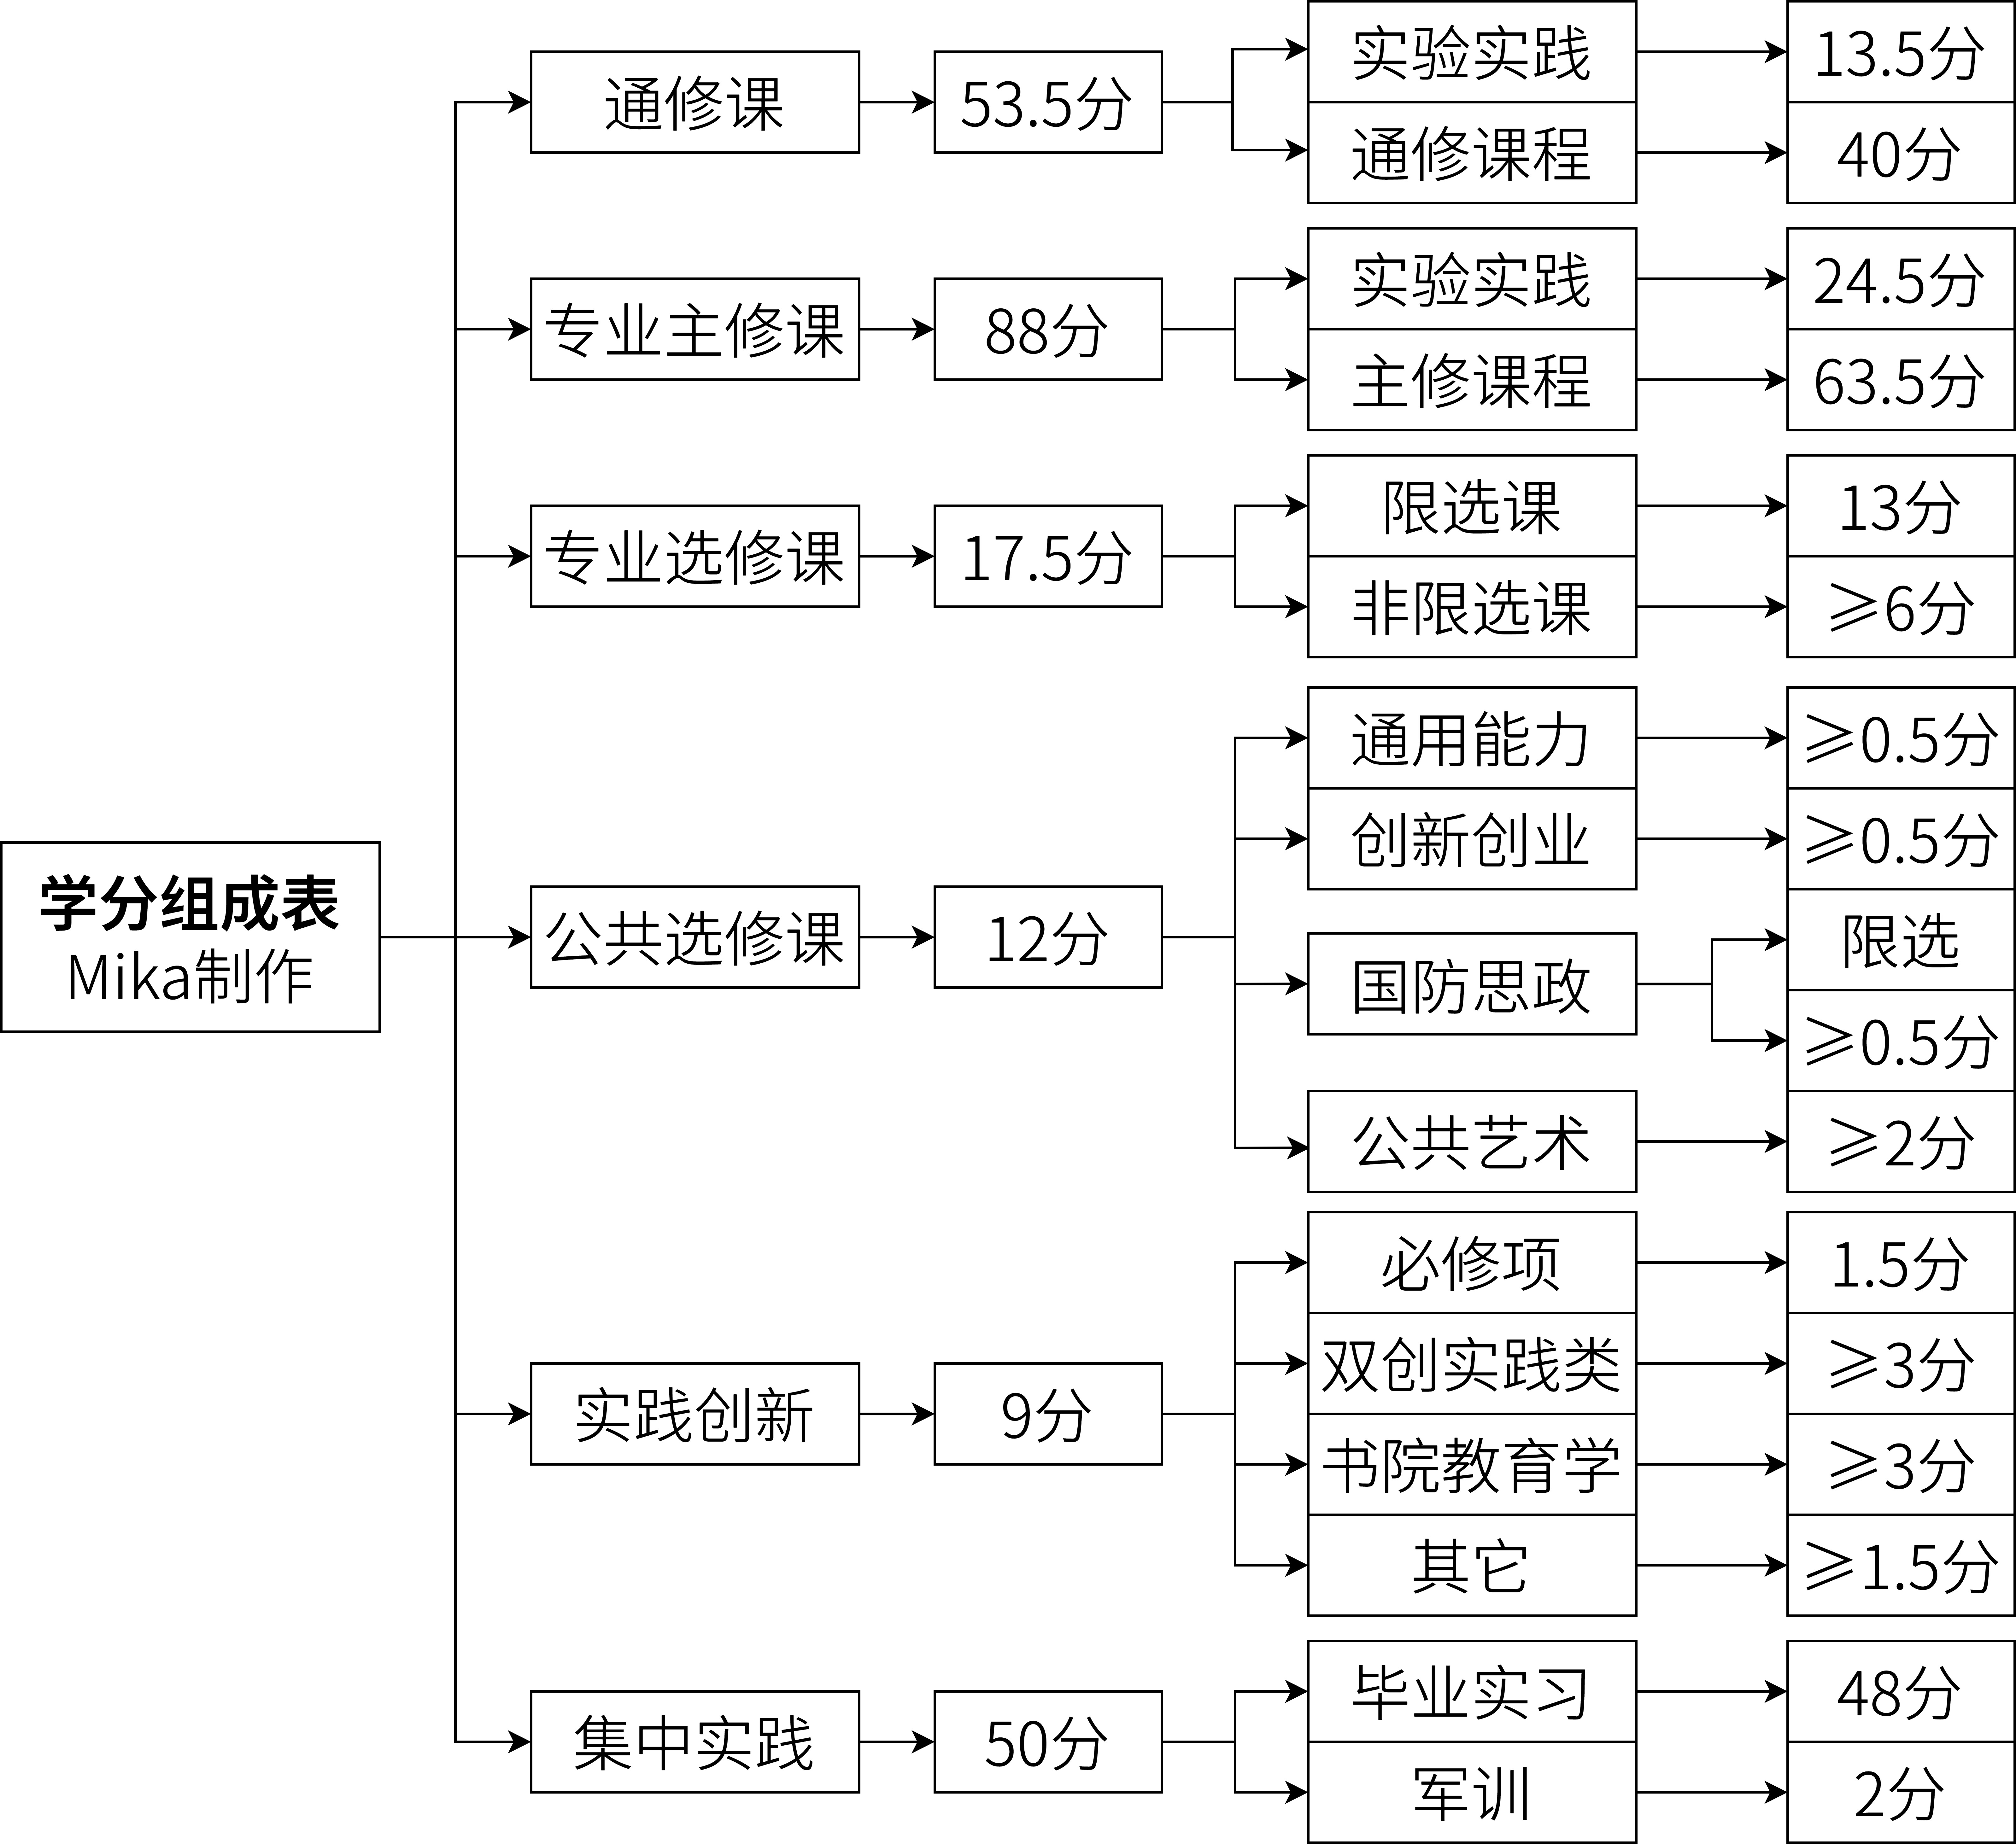
\includegraphics[width=\textwidth]{学分.jpg}
    \caption[学分类别示意图]{学分类别示意图}
\end{table}

\section[学费]{学费}
\begin{enumerate}
    \item 学费收缴工作按照学校财务处通知进行,通常以班级为单位进行通知,可开具电子发票
    \item 如需申请助学贷款、生源地贷款等有特殊情况的同学可咨询学校财务处
    \item 选修课学费按照学分进行收费,所以同一个班的同学学费亦可不同,个人学费以\textbf{“潍坊医学院财务”公众号(潍坊医学院统一支付平台)}中的数据为准
    \item 选修课学分当前规定为1分/100元,多选课多交钱,少选课少交钱(希望大家如果看到了自己希望进一步学习的课程不要吝啬那几百块钱,选课机会只有一次,课程不会重开!)
    \item 此外,一定结合上面的说明修够学分,\textbf{修不够规定学分不能毕业}
\end{enumerate}
%chapter8
\chapter[安全方面]{安全方面}
\vspace{-2em}
\section[用电安全]{用电安全}
\begin{enumerate}
    \item 使用安全的充电器、充电线、插排
    \item 如遇空调、电灯、电风扇等器具出现短路、跳闸、停电等现象时切勿自行维修,请按照\uline{\ref{repair_report}}教程处理
    \item 切勿在宿舍使用冰箱(断电且宿管检查),\textbf{\uuline{如果各位同学需要冷藏保存药物(如胰岛素等),请\\前往大服2楼的药店处}}(地点参见\uline{\ref{common_locations}}),该药店提供付费的低温保存服务
    \item 切勿私改电路,如确有需要,应提前向公寓管理委员\footnotemark 会报备并获得相应许可
    \footnotetext{位于2号公寓南门处。}
    \item 宿舍人走灭灯,无人则关电、切断插座电源
\end{enumerate}

\section[防火安全]{防火安全}
\begin{enumerate}
    \item 切勿使用蚊香以免发生火灾
    \item 切勿在宿舍内烹饪,禁止在宿舍使用各类燃气灶、固体酒精便携灶等易燃易爆危险品
    \item \textbf{禁止在宿舍内吸烟},若实在无法抑制请前往本楼层公共厕所或在宿舍外吸烟完毕后再进宿舍
    \item 请妥善保管打火机、打火石、镁条、火柴等易燃物
\end{enumerate}

\section[出行安全]{出行安全}
\begin{enumerate}
    \item 学校周边基础设施尚在完善建设过程中(\sout{属实是兔葵燕麦、雨井烟垣}),且频繁有货车高速通过。如无特殊情况,\textbf{尽量不要骑公共自行车或者电动车去市里}(泰华城)等,推荐乘坐71路公交车(预计行程30分钟左右)或打车前往
    \item 货车转弯盲区大,极其容易发生安全事故,在等红绿灯时请务必远离“站立禁止区域”
    \item 乘坐出租车(尤其是拼车时)请妥善保管自身财物;如遇失窃请尽快报警,避免正面冲突(谨防持刀伤人)
    \item \textbf{\uuline{严格遵守交通规则,仔细观察周围情况,切忌边看手机边前进,切忌闯红灯}!}
\end{enumerate}

\section[食品安全]{食品安全}
\begin{enumerate}
    \item 如果在餐厅吃坏了肚子或者发现食物质量问题,可前往餐厅一楼东北角的值班室寻求工作人员的帮助
    \item 出现急性腹泻、血便、米泔水样腹泻等情况请尽快前往校医院就诊,切勿拖延
\end{enumerate}

\section[防诈骗及其他注意事项]{防诈骗及其他注意事项}
\begin{enumerate}
    \item \textbf{\uuline{校园贷毁一生,远离高利贷}!}
    \item \textbf{\uuline{杜绝黄赌毒!不要高估自己的意志力}!}
    \item \textbf{刷单就是诈骗!}
    \item 不要贪小便宜乱扫码,信息泄露吃大亏!
    \item 如果碰到一些人自称是市场营销专业、经商专业的,需要卖笔卖本子\footnotemark 才能完成期末考试的,千万不要相信!可以直接联系保卫处
    \footnotetext{{一支批发0.1$¥$的笔卖10$¥$呢,比百乐斑马这种外国牌子都贵,利润高达10000\%……}}
    \item 女生晚上尽量不要独自前往人烟稀少的地方,尤其是西门附近的桃李路等
    \item 谨防诈骗,\textbf{学校永远不会以教务处、学工办的名义,以邮件表格或短信链接的形式通知填写银行卡号和取款密码!}绝对不要相信以“更新银行卡信息”、“填表申请助学金”为由窃取个人资金密码的骗局!如果不确定消息是否属实请致电本班班长,班主任或学工办老师确认
\end{enumerate}

%chapter9
\chapter[衣食住玩与生活]{衣食住玩与生活}
\noindent\textbf{特别声明:}
\begin{enumerate}
    \item 本文中所有\textbf{“大服”},均为\textbf{“大学生服务中心”}的习惯性缩略称呼;
    \item 本文中所有\textbf{“南街”},均为\textbf{“汇金街”}的习惯性缩略称呼。
\end{enumerate}
\section[衣]{衣}
\begin{enumerate}
    \item 大服的2、3层均有服饰商店可自行选购衣物
    \item 推荐网购,也可乘公共汽车前往大型商超购置
    \item 部分院系提供自愿的系服购买服务,详见各院系通知
\end{enumerate}

\section[美食与生活]{美食与生活\footnotemark[1]\footnotemark[2]\footnotemark[3]\footnotemark[4]\footnotemark[5]}
\footnotetext[1]{因文章篇幅原因,本指南仅罗列了同学们提及次数较多的食物或店铺,未能全部列出敬请谅解。}
\footnotetext[2]{下列提及的食物(店铺)均按照空间顺序排列,与好吃程度无关,所用名称为同学习惯性称呼,括号内为特别提醒。}
\footnotetext[3]{标注“$^{〈早〉}$”的店铺约6:00即开始供应。}
\footnotetext[4]{标注“$^{〈晚〉}$”的店铺营业时间最晚可至22:30,其余均在18:30左右停业。}
\footnotetext[5]{奶茶/咖啡店、超市、水果店等单独说明。}

\subsection[大服]{大服}
大服有大量商家提供多种食物,大部分的价格较食堂稍高。
\begin{table}[ht]
    \centering
    \begin{tabular}{|c|c|c|c|c|c|}
        \Xhline{1.2pt}
        \multirow{3}{*}{1层}  & \multirow{2}{*}{内部} & 金小麵$^{〈早〉}$(锅贴)     & 自选菜           & 老陕面馆                   & 馋嘴鱼        \\
        \cline{3-6}
                             &                     & 米粉                  & 肠粉            & 肉夹馍$^{〈晚〉}$            & 冒菜         \\
        \Xcline{2-6}{0.8pt}
                             & 外部                  & 砂锅$^{〈早〉}$(火烧、豆腐脑)  & 大饼卷一切$^{〈晚〉}$ & 速食主义$^{〈早〉}$           & 烧烤$^{〈晚〉}$ \\
        \Xhline{1.2pt}
        \multirow{2}{*}{-1层} & 兰李于                 & 福香面馆$^{〈早〉}$(豆腐脑油条) & 螺狮粉           & 自选菜                    & 蟹王堡        \\
        \cline{2-6}
                             & 烤鸡架                 & 老陕面馆                & 馋嘴鱼           & \multicolumn{2}{c|}{略}              \\
        \Xhline{1.2pt}
    \end{tabular}
\end{table}

\subsection[杏林餐厅]{杏林餐厅}
\vspace{-1em}
杏林餐厅全部三层均有大量食物,大多物美价廉。
\newpage
\begin{table}[ht]
    \centering
    \begin{tabular}{|c|c|c|c|c|}
        \Xhline{1.2pt}
        \multirow{3}{*}{1层} & 麦西麦乐                                                & 包子水饺$^{〈早〉}$ & 牛肉板面                   & 兰州拉面     \\
        \cline{2-5}
                            & 永和豆浆$^{〈早〉}$(油条麻花)                                  & 自选菜(稍贵)      & 豆浆油条                   & 盒饭(便宜量大) \\
        \cline{2-5}
                            & 粥$^{〈早〉}$(种类多)                                      & 馄饨           & 麦西麦乐面包                 & 略        \\
        \Xhline{1.2pt}
        \multirow{3}{*}{2层} & 大骨饭                                                 & 麻汁馄饨         & 水饺                     & 东北玉米面    \\
        \cline{2-5}
                            & 烤鸭饭(瓦罐汤)                                            & 铁板炒饭(量大管饱)   & 清真窗口                   & 茶拌饭      \\
        \cline{2-5}
                            & 馋嘴鱼                                                 & 自选水饺         & \multicolumn{2}{c|}{略}            \\
        \Xhline{1.2pt}
        3层\footnotemark     & \multicolumn{4}{c|}{自选菜(稍贵;小包间式,部门聚餐推荐,包间人数上限为15人)}                                                    \\
        \Xhline{1.2pt}
    \end{tabular}
\end{table}
\footnotetext{仅餐厅东南侧层梯可前往,餐厅东北侧层梯通往原乒乓球场。}

\subsection[汇金街]{汇金街}
\vspace{-1em}
出学校南门,往东一个路口,有大量的饭店,价格较市里相对高昂。
\begin{table}[ht]
    \centering
    \begin{tabular}{|c|c|c|c|c|}
        \Xhline{1.2pt}
        满江红 & 石锅鱼 & 暖溢水饺 & 幸福餐厅 & 小四川 \\
        \Xhline{1.2pt}
    \end{tabular}
\end{table}

\subsection[超市]{超市}\label{market}
\begin{table}[ht]
    \centering
    \begin{tabular}{|c|c|c|}
        \Xhline{1.2pt}
        习惯称呼         & 地点      & 物品                   \\
        \Xhline{1.2pt}
        大服超市$^{〈晚〉}$ & 在大服正中央  & 日用品,零食,饮料,手套,头套,作业本等 \\
        \hline
        中和超市         & 中和广场    & 日用品(少)、零食、饮料等        \\
        \hline
        餐厅超市         & 餐厅西北侧入口 & 零食、饮料等               \\
        \Xhline{1.2pt}
    \end{tabular}
\end{table}

\subsection[水果店]{水果店}
\begin{table}[!ht]
    \centering
    \begin{tabular}{|c|c|c|c|c|c|}
        \Xhline{1.2pt}
        习惯称呼    & 地点                     & 种类 & 新鲜   & 价格 \\
        \Xhline{1.2pt}
        餐厅南水果店  & 餐厅正南侧入口                & 较多 & 较好   & 略高 \\
        \hline
        餐厅西水果店  & 餐厅正西侧入口                & 较少 & 一般   & 一般 \\
        \hline
        大服水果店   & 大服西南侧                  & 最多 & 一般或好 & 最高 \\
        \hline
        中和/大服超市 & 见 \uline{\ref{market}} & 最少 & 一般   & 最低 \\
        \Xhline{1.2pt}
    \end{tabular}
\end{table}

\subsection[奶茶/咖啡店]{奶茶/咖啡店}
\begin{table}[!ht]
    \centering
    \begin{tabular}{|c|c|c|c|c|c|}
        \Xhline{1.2pt}
        \multirow{3}{*}{食堂} & \multirow{2}{*}{内部} & 蜜雪冰城 & 沪上阿姨  & 阿水大杯茶                             & 麦克风          \\
        \cline{3-6}
                            &                     & 小度   & 冰雪岛   & 超级奶爸                              & $\backslash$ \\
        \cline{2-6}
                            & 外部                  & 潍医咖啡 & 臻茶    & \multicolumn{2}{c|}{$\backslash$}                \\
        \Xhline{1.2pt}
        \multirow{2}{*}{大服} & 1层                  & 茶百道  & 益禾堂   & \multicolumn{2}{c|}{$\backslash$}                \\
        \cline{2-6}
                            & 2层                  & 库迪咖啡 & 遇觅烧仙草 & \multicolumn{2}{c|}{$\backslash$}                \\
        \Xhline{1.2pt}
    \end{tabular}
\end{table}

\newpage
\subsection[其他常用地点]{其他常用地点}
\begin{table}[!ht]
    \vspace{-1em}
    \centering
    \begin{tabular}{|c|c|c|c|}
        \Xhline{1.2pt}
        地点                    & 习惯称呼               & 位置     & 功能                        \\
        \Xhline{1.2pt}
        \multirow{9}{*}{大服}   & 厕所                 & -1层东北  & 略                         \\
        \cline{2-4}
                              & 联通营业厅              & 1层超市旁  & 联通业务办理                    \\
        \cline{2-4}
                              & 药店、牙科              & 2层西北   & 买药、看牙、\textbf{冷藏药品}       \\
        \cline{2-4}
                              & 理发店(两家)            & 2层     & 烫染剪发                      \\
        \cline{2-4}
                              & 复印店(两家)            & 2层     & 复印、证件照、复习资料购买             \\
        \cline{2-4}
                              & 干洗店                & 2层东    & 干洗、实验服购买、配钥匙              \\
        \cline{2-4}
                              & 维修店                & 2层东南   & 手机电脑维修、手机配件购买             \\
        \cline{2-4}
                              & \textbf{办公室}       & 2层东北   & 水卡的办卡充值退卡                 \\
        \cline{2-4}
                              & 大服健身房\footnotemark & 3层     & 运动健身、办理健身会员卡              \\
        \cline{2-4}
                              & 台球厅\               & 3层     & 打台球                       \\
        \Xhline{1.2pt}
        \multirow{3}{*}{中和广场} & 学生印务               & A106对过 & 打印、复印、\textbf{复习资料购买、二手书} \\
        \cline{2-4}
                              & 移动营业厅              & A104对过 & 移动业务办理                    \\
        \cline{2-4}
                              & 邮政银行ATM            & A103对过 & 存取款                       \\
        \Xhline{1.2pt}
        \multirow{4}{*}{其他}   & 证件照                & B207旁  & 证件照、特殊复印(80g/120g纸)       \\
        \cline{2-4}
                              & \textbf{证明打印}      & D105旁  & \textbf{学籍证明、成绩证明}等       \\
        \cline{2-4}
                              & 自助打印               & 餐厅北侧   & 打印                        \\
        \cline{2-4}
                              & 二手书购买              & 7号宿舍西南 & 二手书售卖(大量)                 \\
        \Xhline{1.2pt}
    \end{tabular}
    \footnotetext{仅大服西北侧楼梯可前往。}
\end{table}

\section[住]{住}
\begin{enumerate}
    \item 宾馆:南街提供大量宾馆、客房等
    \item 自习室:南街部分宾馆提供通宵自习服务
    \item 出租房:附近小区由较多房屋出租\footnotemark
\end{enumerate}
\footnotetext{须在学校办理走读手续后才可在外居住。}

\section[玩]{玩}
\begin{enumerate}
    \item 多数同学常通过步行前往南街,有KTV、电影院等娱乐场所
    \item 可通过69、71路公交车(北门乘坐)或13、109路公交车(南门乘坐)前往市区(如泰华、万达、谷德茂等)进行游玩
    \item 校内的文体中心\footnotemark(位置见\ref{map_a})内有羽毛球馆、篮球馆(两者互斥\footnotemark)、健身房,还有\textbf{游泳馆}等
    \footnotetext{具体收费标准及预约方式见下文\uline{text}}
    \footnotetext{详见本文章\uline{\href{https://mp.weixin.qq.com/s/n0Tc7LL3OCfyALKUUxrs9Q}{https://mp.weixin.qq.com/s/n0Tc7LL3OCfyALKUUxrs9Q}}}
\end{enumerate}

\end{document}